\documentclass[11pt, a4paper, oneside]{report}
\usepackage[utf8]{inputenc}
\usepackage{graphicx}
\usepackage[english]{babel}
\usepackage{float}
\usepackage{draculatheme}
\usepackage{enumitem}
\usepackage[top=1in, bottom=1.25in, left=1.25in, right=1.25in]{geometry}
\renewcommand{\familydefault}{\ttdefault}

\pagestyle{empty}

\title{Standard Work Instructions for Nesting with Radan for the Mitsubishi Laser}
\author{Justin Wayne Liles \thanks{Approved by *}}
\date{04.March.2022}

\begin{document}
\renewcommand{\labelenumii}{\arabic{enumi}.\arabic{enumii}}
\renewcommand{\labelenumiii}{\arabic{enumi}.\arabic{enumii}.\arabic{enumiii}}
\renewcommand{\labelenumiv}{\arabic{enumi}.\arabic{enumii}.\arabic{enumiii}.\arabic{enumiv}}
\begin{titlepage}
    \maketitle
\end{titlepage}
\textbf{This is an SWI for the \emph{Mitsubishi Laser.}}
\begin{enumerate}
    \item Ensure proper machine tooling before initializing a new nest.
        \begin{figure}[!h]
            \centering`
            \descriptionlabel{Confirm machine tooling by looking at the window title bar}
            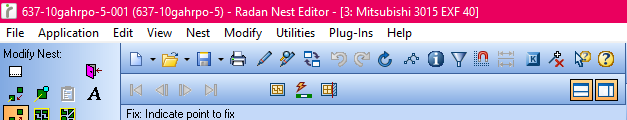
\includegraphics[width=12cm]{/home/jwl/projects/swi/Resources/verify-tooling.png}

            \caption{Confirm machine tooling by looking at the window title bar}
        \end{figure}
        \begin{enumerate}
            \item How to adjust tooling.
                \begin{figure}[!h]
                    \centering
                    \descriptionlabel{Change Machine Tooling Menu Location}
                    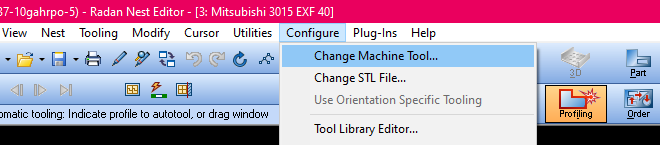
\includegraphics[width=12cm]{/home/jwl/projects/swi/Resources/change-tooling.png}
                    \caption{You \emph{MUST} be in the Profiling tab to access this menu}
                \end{figure}
                \begin{enumerate}
                    \item Select the correct tooling for the laser being nested.
                        \begin{figure}[!h]
                            \centering
                            \descriptionlabel{Machine List Dialog}
                            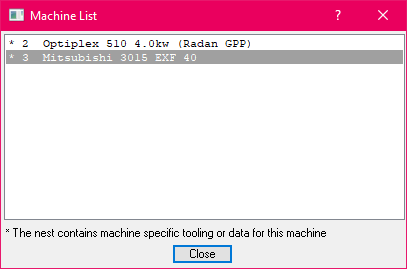
\includegraphics[width=12cm]{/home/jwl/projects/swi/Resources/select-tooling.png}
                            \caption{Select Tool - * 3 Mitsubishi 3015 EXF 40}
                        \end{figure}
                        \newpage
                    \item Verify the tooling has changed.
                        \begin{figure}[!h]
                            \centering
                            \descriptionlabel{Tooling Change Notification}
                            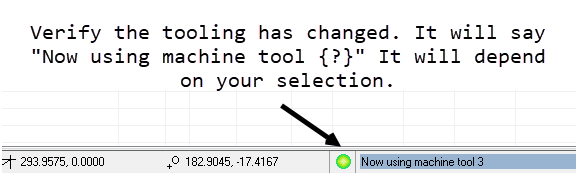
\includegraphics[width=12cm]{/home/jwl/projects/swi/Resources/tooling-change-notification.png}
                            \caption{Look at the status bar to confirm the tooling has changed}
                        \end{figure}
                \end{enumerate}
        \end{enumerate}
    \item Initialize a new Project.
        \begin{enumerate}
            \item Explain how and why we title Projects.
                \begin{enumerate}
                    \item Each programmer has a number used as an identifier.
                \end{enumerate}
            \item Saving the Project.
                \begin{enumerate}
                    \item Ensure that the default locations are set correctly.
                        \begin{enumerate}
                            \item Explain how to reset the default save locations if they have been modified.
                        \end{enumerate}
                \end{enumerate}
            \item Explain the difference between initializing a new Project from the "system default" vs. "current Project."
                \begin{enumerate}
                    \item The use of the current Project is helpful if making multiple nests from the same material.
                \end{enumerate}
        \end{enumerate}
    \item Explain how to set material and sheet size.
        \begin{enumerate}
            \item How to select the correct material and sheet size.
                \begin{enumerate}
                    \item Which thickness options to use for each type of material? The thickness of the material options listed does not match the thickness of the materials being cut.
                \end{enumerate}
            \item Scrap material.
                \begin{enumerate}
                    \item How to set non-standard sheet sizes in the sheet schedule.
                \end{enumerate}
        \end{enumerate}
    \item How to add parts to the parts schedule.
        \begin{enumerate}
            \item Explain the part selection process.
                \begin{enumerate}
                    \item Which folder is used to select parts?
                    \item Make sure that the symbols used are for the correct machine. For example, some symbols are explicitly made for the Mitsubishi to be easier to shake out or designed for common line nesting to increase utilization per sheet.
                    \item How to add multiple parts simultaneously.
                \end{enumerate}
            \item Set priority per part.
                \begin{enumerate}
                    \item Explain how the priority setting affects the nesting process and how to use it to ensure higher utilization per sheet.
                \end{enumerate}
            \item Explain required qty vs. extra qty.
                \begin{enumerate}
                    \item Explain how this setting can also assist with getting a higher utilization per sheet.
                \end{enumerate}
            \item General nesting process.
                \begin{enumerate}
                    \item This section is for any general advice or miscellaneous information involving the nesting process.
                \end{enumerate}
        \end{enumerate}
    \item Adjust multi-part nesting settings.
        \begin{enumerate}
            \item Set "Nesting Options"
                \begin{enumerate}
                    \item We can modify the allowed time per nest to allow Radan more nesting attempts before moving onto the following program.
                    \item The SWI will explain other options at this time as well.
                \end{enumerate}
            \item Set "Clearances"
                \begin{enumerate}
                    \item What measurements to use at each gap.
                    \item Explain the reasons for each measurement.
                \end{enumerate}
            \item Set "Automatic Order" in the Automation Tab.
                \begin{enumerate}
                    \item Which Automatic Order option to select.
                    \item Why the Automation is not effective with the Mitsubishi laser.
                \end{enumerate}
        \end{enumerate}
    \item Run the nester.
        \begin{enumerate}
            \item General information on what to watch for while the nester is running.
                \begin{enumerate}
                    \item Watch the parts schedule to see when parts are being nested.
                \end{enumerate}
            \item How to stop the nester while running.
                \begin{enumerate}
                    \item How to stop the nester and why a nest is determined to be inefficient or unnecessary before Radan completing the process.
                \end{enumerate}
        \end{enumerate}
    \item Check the nests.
        \begin{enumerate}
            \item Check the Utilization.
                \begin{enumerate}
                    \item Explain when a lower utilization is acceptable and set a time limit for seeking a higher utilization.
                        \begin{enumerate}
                            \item Do not spend excessive time to improve utilization only.
                        \end{enumerate}
                \end{enumerate}
            \item Check the programs.
                \begin{enumerate}
                    \item Confirm that needed parts are nested.
                    \item Confirm the nest is using as few sheets as needed.
                        \begin{enumerate}
                            \item Reducing the nest size to keep close to the needed parts rather than bloating a nest with low-priority parts.
                        \end{enumerate}
                \end{enumerate}
        \end{enumerate}
    \item Set Automatic Tooling.
        \begin{enumerate}
            \item Pick the correct strategy.
                \begin{enumerate}
                    \item Which strategy for each sheet thickness. \textbf{Note:} The Mitsubishi currently cuts all material less than .250" with Nitrogen. Air is not to be used until otherwise told.
                    \item The strategy guide is this:
                        \begin{enumerate}
                            \item Use Air if the material is equal to or less than 0.080.
                            \item Use Nitrogen if the material is greater than 0.080 and equal to or less than .250.
                            \item Otherwise, use Oxygen.
                        \end{enumerate}
                \end{enumerate}
        \end{enumerate}
    \item Set proper tags.
        \begin{enumerate}
            \item Explain when tags may be needed or not needed. The larger the gauge or thickness of a material, the less likely it is to need tags. No tags also make it easier to shake out the heavier parts.
        \end{enumerate}
    \item Set "Rules and Styles"
        \begin{enumerate}
            \item Currently, it is unknown to me why a specific style is chosen over any other. However, looking through the styles leads me to believe that the selected styles have the highest drawing and rapid speeds. Therefore, I will investigate this step further.
        \end{enumerate}
    \item Set Sheet Scrapping and Offcuts.
        \begin{enumerate}
            \item Add scrap cuts and scrap cut spacing.
                \begin{enumerate}
                    \item Explain the options contained in the prompt.
                    \item Add offcuts if cutting non-standard sheet size.
                \end{enumerate}
        \end{enumerate}
    \item Set the cut order.
        \begin{enumerate}
            \item Select the correct Order Style.
                \begin{enumerate}
                    \item I will research more about this aspect of Radan nesting.
                \end{enumerate}
            \item Set the bottom right corner piece as the first to cut to allow the operator to check the cut before letting the sheet run.
        \end{enumerate}
    \item Compile the program.
        \begin{enumerate}
            \item These options are generally set in the actions described above. In addition, this prompt allows for reviewing the conditions before compiling.
                \begin{enumerate}
                    \item When OK is selected, the compilation process will start. Upon completion, choose OK to return to the workspace.
                \end{enumerate}
        \end{enumerate}
    \item Save the Project.
        \begin{enumerate}
            \item After completing the compilation process, save the resultant blocks file.
                \begin{enumerate}
                    \item Explain where to save and how to title the programs.
                \end{enumerate}
            \item Take a screen capture of the workspace to use as a cover sheet for the Project when carried out to the laser.
        \end{enumerate}
    \item Push the Project to the correct laser.
        \begin{enumerate}
            \item Explain to which folder a copy of the Project belongs.
        \end{enumerate}
    \item Print the orders.
        \begin{enumerate}
            \item Use the screen capture to print the orders as needed.
                \begin{enumerate}
                    \item Some of the orders will need to have qty, material, or work center changed.
                        \begin{enumerate}
                            \item Sometimes, we will move orders from its original work center to the laser for a faster turnaround.
                            \item There will be occasions where a part number has multiple orders that are urgent. It is good practice to combine these orders to prevent confusion.
                        \end{enumerate}
                \end{enumerate}
        \end{enumerate}
    \item Carry the Project packet out to the laser and let the operator know it is there.
\end{enumerate}
\end{document}
